% !TEX encoding = UTF-8
% !TEX TS-program = pdflatex
% !TEX root = rel_datamining.tex
% !TEX spellcheck = it-IT

\section{Elaborazione delle variabili}

Il dataset si presenta con poche variabili che riassumono molte informazioni o che hanno un numero molto elevato di livelli. \`E quindi necessario andare ad estrapolare le informazioni da queste variabili, creandone di nuove e di più semplici.

\subsection{Il nome dell'animale}

La variabile \texttt{Name} ha più di 6000 possibili valori distinti e, ragionando a livello di previsione, sembra poco probabile che il nome dell'animale influisca sul suo destino. Tuttavia ci sono 7691 animali che non hanno un nome, questo probabilmente implica che si tratta di animali randagi che sono stati portati al rifugio\footnote{Non vengono fornite informazioni a riguardo} e quindi può essere meno probabile che il padrone li venga a recuperare. Analogamente se è stato trovato un'animale smarrito e con una targhetta con il nome al collo, è più probabile che il suo padrone vada a recuperarlo.

Il nome può quindi essere riassunto da una nuova variabile booleana \texttt{HasName} che specifica se l'animale ha un nome o meno.

Tracciando il grafico (Figura \ref{fig-has-name}) per visualizzare la ripartizione delle varie classi per la variabile risposta in base al valore di \texttt{HasName} si ha che le osservazioni fatte sembrano essere confermate dai dati: indipendentemente dal tipo di animale, se questo ha un nome è più probabile che venga recuperato dal suo padrone. Inoltre, si può notare anche che per i gatti, la probabilità di essere adottati è molto più alta se hanno un nome.

\begin{figure}[htbp]
	\centering
	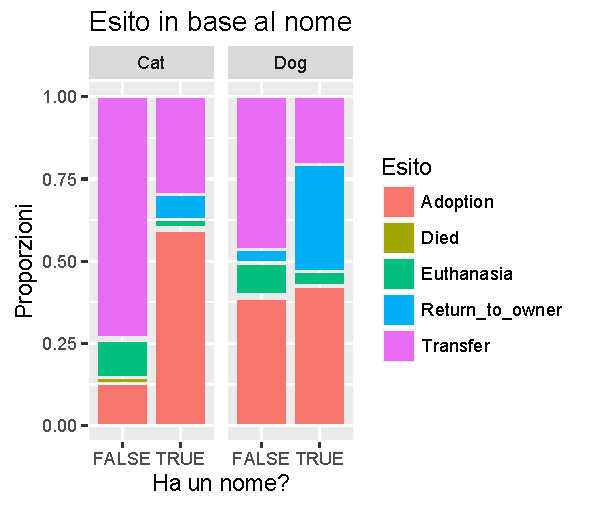
\includegraphics[width=0.5\textwidth]{./grafici/esito_has_name.pdf}
	\caption{Esito in base al nome}\label{fig-has-name}
\end{figure}

\subsection{La data di uscita}

Difficilmente la data in cui l'animale ha lasciato la struttura può tornare utile per effettuare previsioni future. Si possono però estrarre altre informazioni come la fascia oraria e il giorno della settimana in cui l'animale ha lasciato la struttura. 

Queste due informazioni possono tornare utili perché, ad esempio la gente nei week-end ha più tempo libero e quindi è più probabile che vada ad adottare un animale, oppure che per motivi logistici i trasferimenti possono essere fatti solamente la mattina.

Per estrapolare ciò vengono definite due nuove variabili \texttt{DayOfWeek} che assume come valore il giorno della settimana e \texttt{TimeOfDay} che può assumere come valori:

\begin{itemize}
	\item \textit{Mattina}: se l'ora è compresa tra le 6 e le 12.
	\item \textit{Pomeriggio}: se l'ora è compresa tra le 12 e le 17.
	\item \textit{Sera}: se l'ora è compresa tra le 17 e le 20.
	\item \textit{Notte}: per le restanti ore.
\end{itemize}

Come si può notare dal grafico (Figura \ref{fig-time}) c'è un picco sulle adozioni nella fascia serale. Sempre dal grafico si può notare che la notte sono più frequenti i trasferimenti, anche se la maggior parte di questi si viene svolta durante le ore diurne, questo perché l'attività notturna del rifugio è molto limitata (423 osservazioni).

\begin{figure}[htbp]
	\centering
	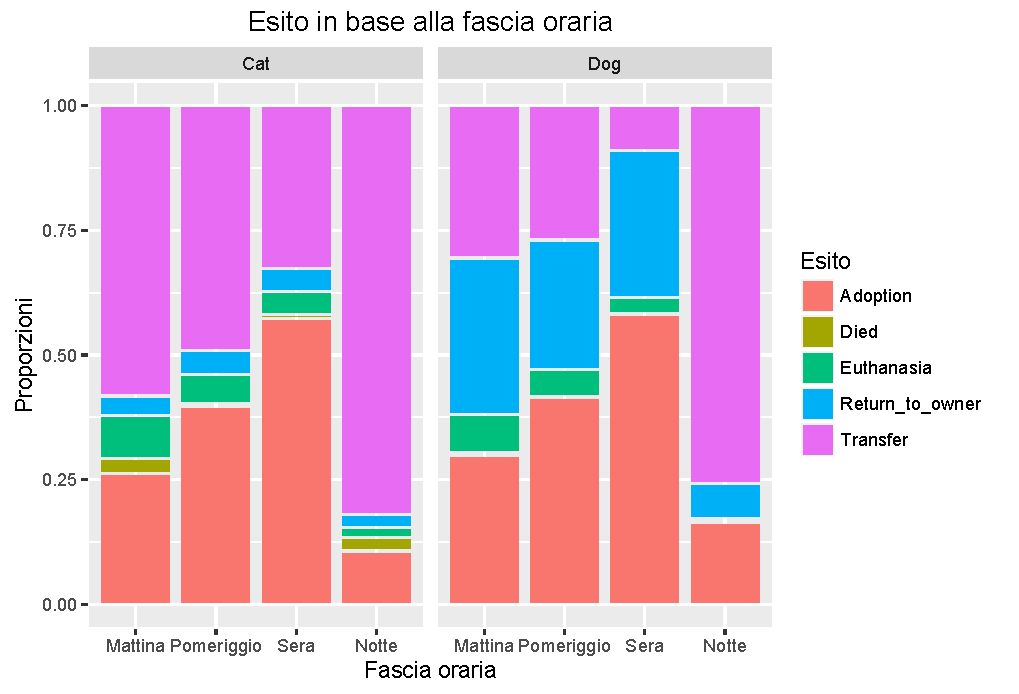
\includegraphics[width=0.6\textwidth]{./grafici/esito_time.pdf}
	\caption{Esito in base alla fascia oraria}\label{fig-time}
\end{figure}

Per quanto riguarda il giorno della settimana, dal grafico Figura \ref{fig-dow}, si può notare come le adozioni siano leggermente più probabili nel week-end.

\begin{figure}[htbp]
	\centering
	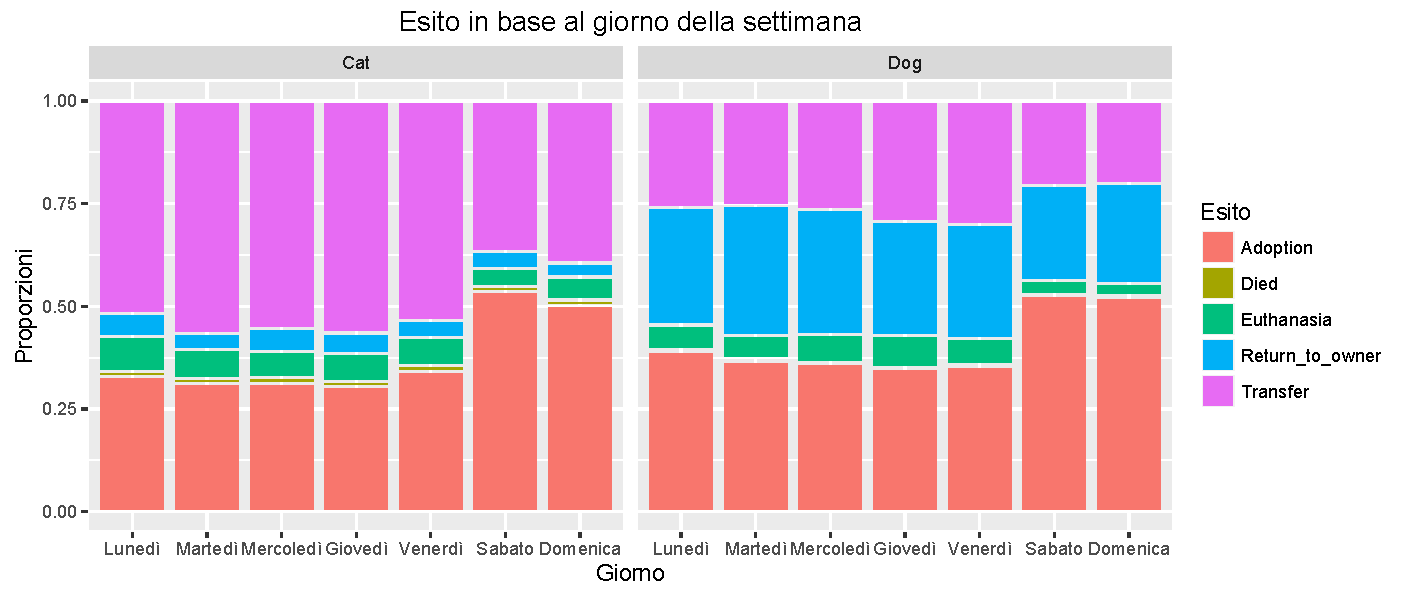
\includegraphics[width=0.9\textwidth]{./grafici/esito_week.pdf}
	\caption{Esito in base al giorno della settimana}\label{fig-dow}
\end{figure}

\subsection{Sesso e stato dell'animale}

La variabile \texttt{SexuponOutcome} prevede 6 possibili livelli che racchiudo l'informazione relativa al sesso e al fatto se l'animale è stato sterilizzato o meno. C'è poi un livello \textit{Unknown} per gli animali per i quali non si hanno informazioni e in più ci sono dei valori \texttt{NA}.

Questa variabile è stata quindi scomposta in \texttt{Gender} che specifica il sesso dell'animale e \texttt{Status}, che specifica se l'animale è stato sterilizzato o meno. Entrambe le variabili hanno un terzo possibile valore \textit{Unknown} che rappresenta la mancanza di informazioni.

Dal grafico riportato in Figura \ref{fig-sesso-stato} si può notare che indipendentemente dal sesso e dal tipo di animale, se l'animale è stato sterilizzato è più probabile che venga adottato. Se invece non è stato sterilizzato oppure non ci sono informazioni a riguardo, è più probabile che venga trasferito.

\begin{figure}[htbp]
	\centering
	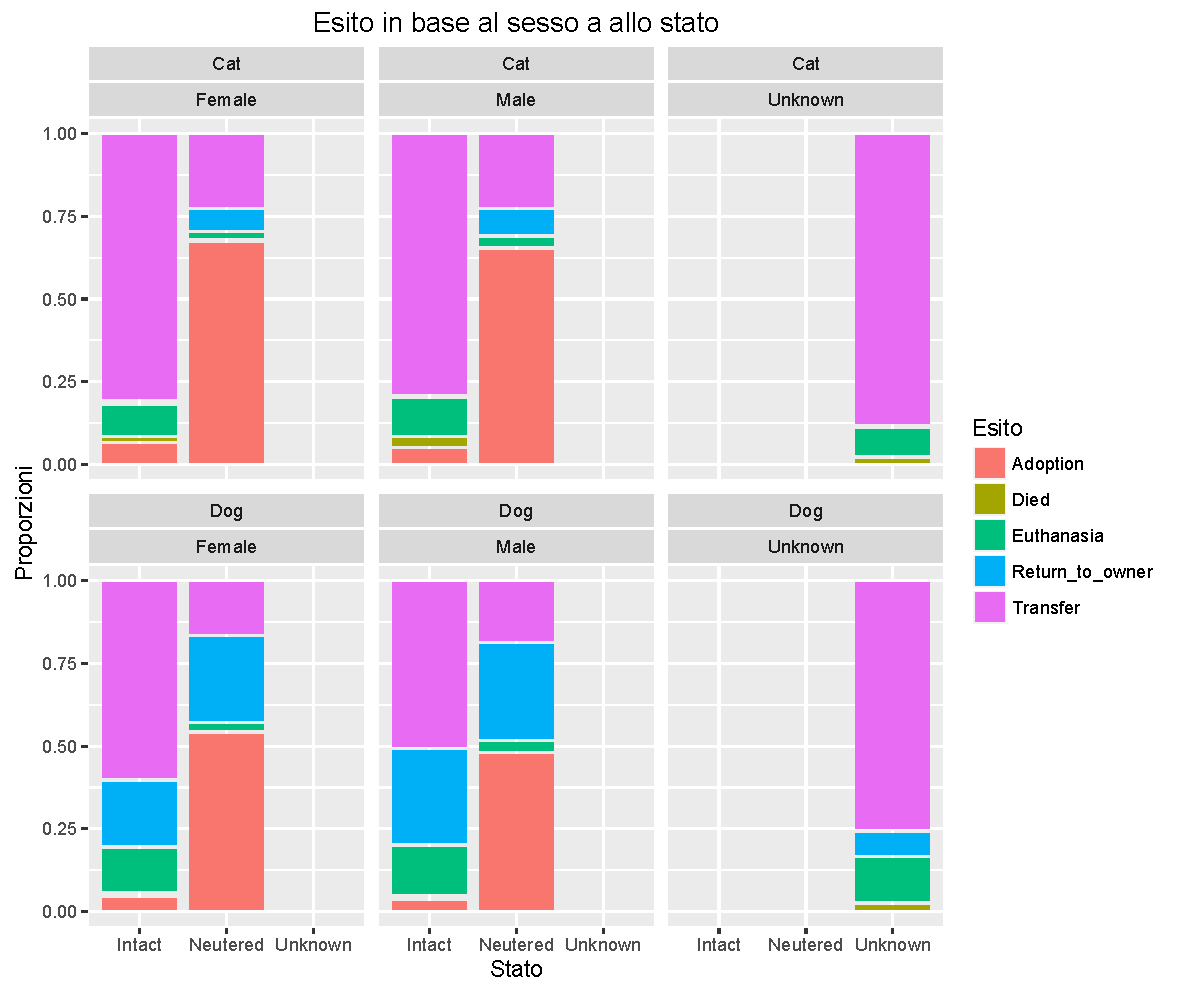
\includegraphics[width=0.8\textwidth]{./grafici/esito_sesso_stato.pdf}
	\caption{Esito in base al sesso e allo stato dell'animale}\label{fig-sesso-stato}
\end{figure}

\subsection{L'età dell'animale}

L'età dell'animale è memorizzata nella variabile \texttt{AgeuponOutcome} in un formato molto confusionale in quanto viene espressa come \textit{2 anni}, \textit{3 mesi}, ecc. Inoltre ci sono dei casi in cui alcuni valori non hanno la \textit{s} del plurale, ovvero tra i possibili valori della variabile ci sono ad esempio \textit{1 week} e \textit{1 weeks}, che quindi vengono considerati come valori distinti quando in realtà non lo sono.

La prima modifica è quindi quella di normalizzare i valori, esprimendoli con un numero intero che approssima l'età dell'animale espressa in giorni. Così facendo risulta più semplice classificare gli animali per fascia d'età. Infatti, si può assumere che un cucciolo è più probabile che venga adottato rispetto ad un animale più anziano, mentre gli animali troppo piccoli non possono essere adottati per legge.

Conviene quindi creare una nuova variabile \texttt{AgeCategory} con 5 possibili livelli:

\begin{itemize}
	\item \textit{Neonato}: da 0 a 29 giorni.
	\item \textit{Cucciolo}: da 30 a 365 giorni.
	\item \textit{Adulto}: da 366 a 3650 giorni (10 anni).
	\item \textit{Anziano}: più di dieci anni.
	\item \textit{Sconosciuta}.
\end{itemize}

Nella normalizzazione dei valori si è scelto di mantenere le 18 osservazioni con i valori mancati per l'età, marcandoli come sconosciuti, questo perché nel secondo dataset sono presenti delle osservazioni per le quali l'eta non è nota. Inoltre, si può ipotizzare che questi animali siano randagi e quindi che per questo motivo la loro eta non è nota.
Questa ipotesi deriva dal fatto che tra i possibili valori della variabile \texttt{OutcomeSubtype} c'è il valore \textit{SCRP} che indica un trasferimento relativo al programma di recupero dei gatti randagi\footnote{\url{http://www.maddiesfund.org/austin-animal-services-stray-cat-return-program.htm}} e quasi tutte le osservazioni con l'età mancante hanno proprio quel valore come \texttt{OutcomeSubtype}.

\begin{figure}[htbp]
	\centering
	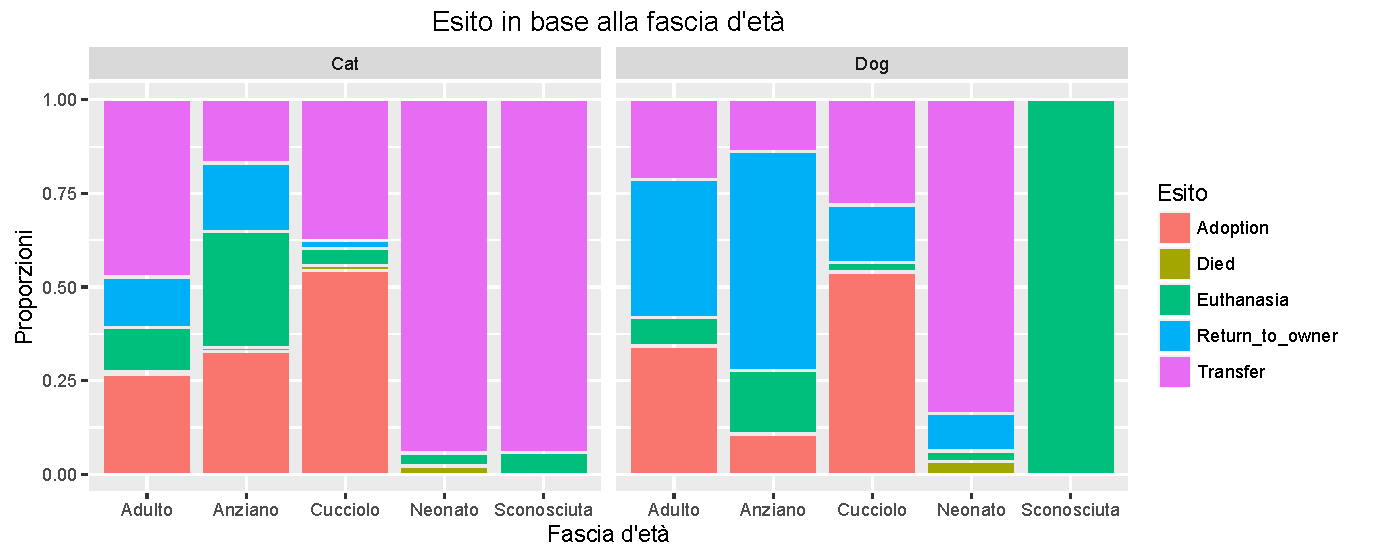
\includegraphics[width=0.9\textwidth]{./grafici/esito_eta.pdf}
	\caption{Esito in base alla fascia d'età dell'animale}\label{fig-eta}
\end{figure}

Come si può notare dal grafico Figura \ref{fig-eta}, nessuno degli animali neonati viene adottato ed è più probabile che vengano trasferiti. Per quanto riguarda la probabilità di adozione, questa è maggiore per i cuccioli e più bassa per i cani anziani. I gatti anziani hanno una maggiore probabilità di adozione rispetto ai cani anziani e questo può essere dovuto al fatto che la speranza di vita di un gatto è maggiore rispetto a quella di un cane.

\subsection{Razza}

Le informazioni relative alla razza dell'animale sono racchiuse nella variabile \texttt{Breed}, la quale ha 1340 possibili valori e specifica anche se l'animale è un incrocio o meno.

Osservando alcuni dei possibili valori, si può notare che se l'animale non è di razza, il valore della variabile comprende o due razze oppure la razza principale seguita da \textit{Mix}. Si è scelto quindi di scomporre la variabile \texttt{Breed} nelle variabili \texttt{PrimaryBreed} (220 livelli), \texttt{SecondaryBreed} (144 livelli) e \texttt{IsMix} (booleana).

Ci sarebbero ulteriori informazioni che possono essere estratte da questa variabile, come la stazza dell'animale, la quale a sua volta va ad influire sull'aspettativa di vita e quindi sulla corretta classificazione della fascia d'età e sul carattere dell'animale. Tuttavia per estrarre queste informazioni in modo corretto è necessaria un'elevata conoscenza del dominio, ci si è quindi limitati alla scomposizione della variabile \texttt{Breed}.

\begin{figure}[htbp]
	\centering
	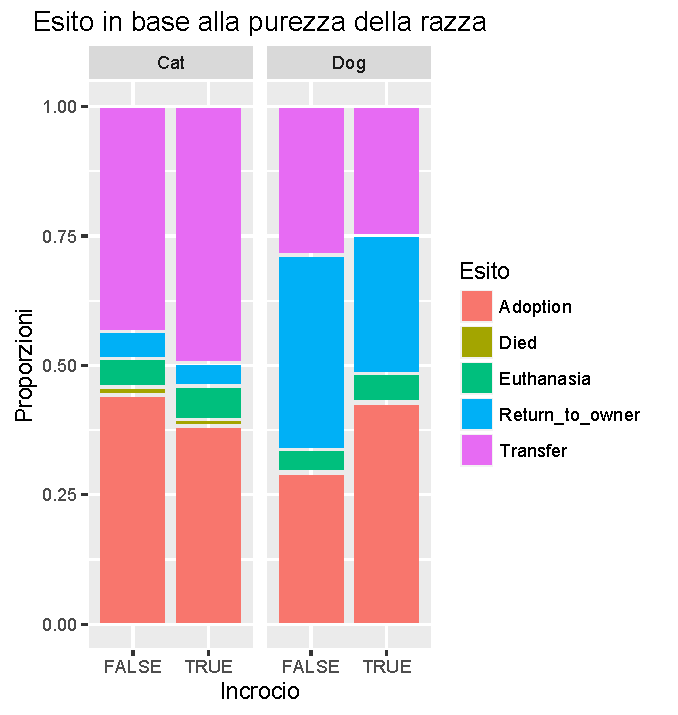
\includegraphics[width=0.5\textwidth]{./grafici/esito_mix.pdf}
	\caption{Esito in base alla fascia d'età dell'animale}\label{fig-mix}
\end{figure}


Come si può notare dal grafico in Figura \ref{fig-mix}, un cane di razza ha più probabilità di essere adottato rispetto ad un cane non di razza, mentre per i gatti sembra che avvenga il contrario. Non sono stati inseriti i grafici per le variabili \texttt{PrimaryBreed} e \texttt{SecondaryBreed} perché il numero elevato di possibili valori li rende incomprensibili.

\subsection{Colore}

Come per la razza, anche per il colore le informazioni sono racchiuse nell'unica variabile \texttt{Color} e, sempre come per la razza, queste informazioni sono state suddivise nelle variabili:

\begin{itemize}
	\item \texttt{PrimaryColor}: colore principale, 29 livelli.
	\item \texttt{SecondaryColor}: colore secondario, 24 livelli.
	\item \texttt{Pattern}: pattern del pelo, 10 livelli.
	\item \texttt{HasComplexColor}: valore booleano che specifica se il pelo dell'animale ha più colori o un certo pattern particolare.
\end{itemize}

Sarebbe poi necessario andare a normalizzare i valori dei colori, dato che ci sono più livelli che indicano lo stesso colore, come \textit{Orange} e \textit{Apricot} (albicocca), ma da una prima analisi grafica (Figura \ref{fig-colors}) sembra che, stabilito il tipo di animale, le informazioni sul colore non influiscano sull'esito e in quei pochi casi che questo succede può essere dovuto al fatto che si hanno troppe poche osservazioni con quel determinato colore.

\begin{figure}[!ht]
	\centering
	\subfloat{%
		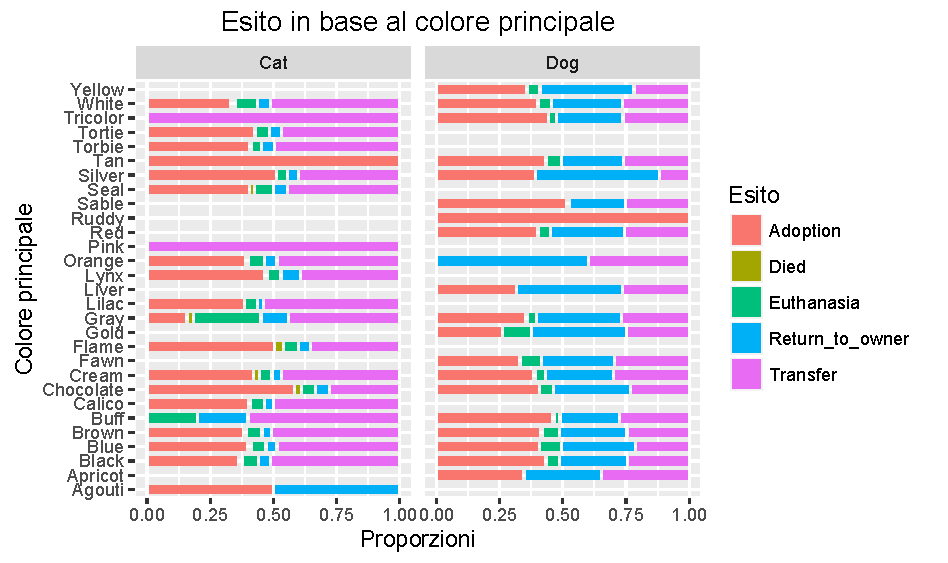
\includegraphics[width=0.48\textwidth]{./grafici/esito_colore_principale.pdf}
	}
	\quad
	\subfloat{%
		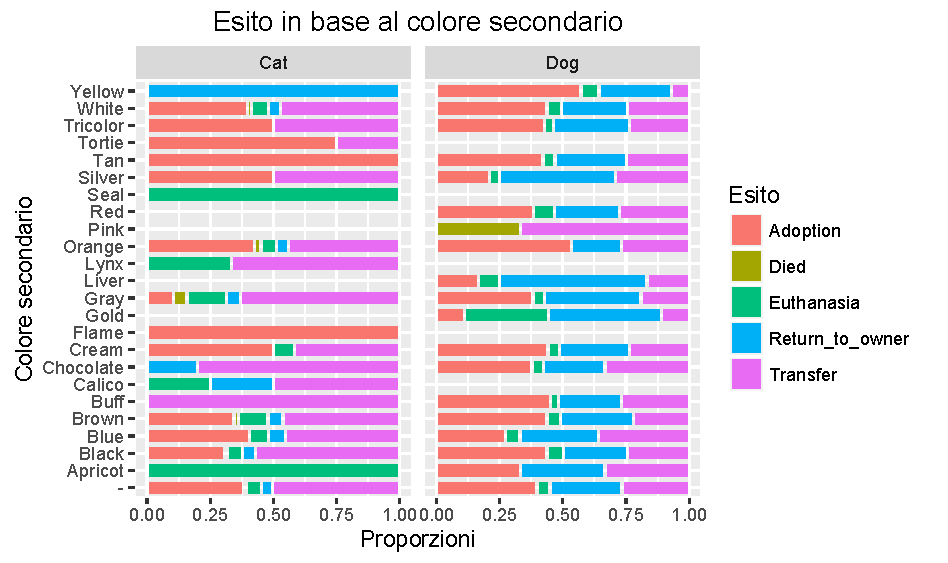
\includegraphics[width=0.48\textwidth]{./grafici/esito_colore_secondario.pdf}
	}
	
	\subfloat{%
		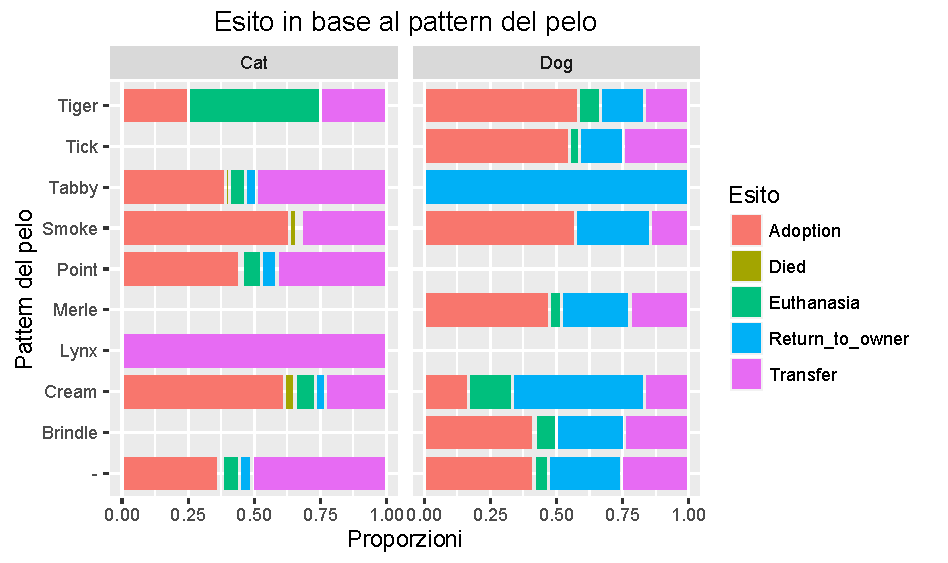
\includegraphics[width=0.48\textwidth]{./grafici/esito_pattern.pdf}
	}   
	\quad
	\subfloat{%
		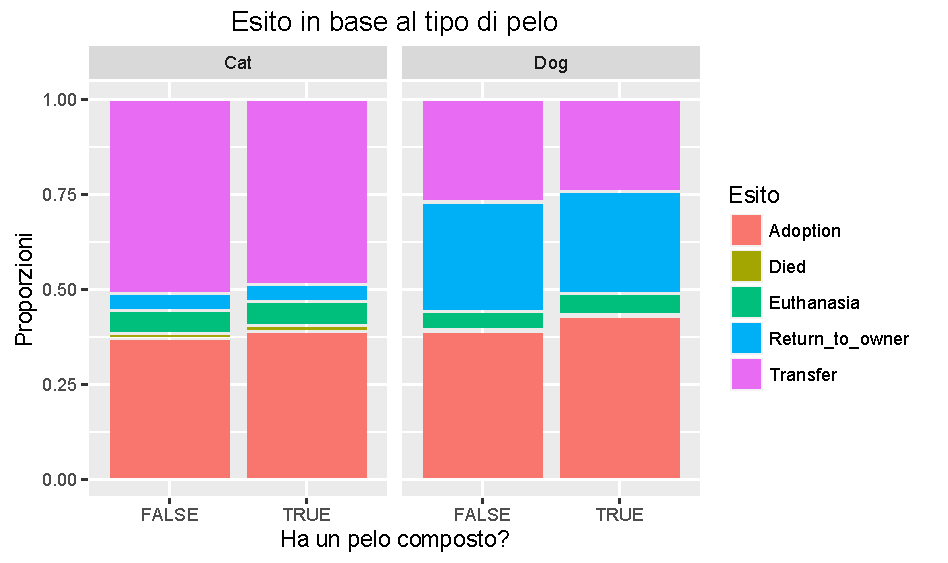
\includegraphics[width=0.48\textwidth]{./grafici/esito_has_complex_color.pdf}
	}
	\caption{I grafici della prima riga rappresentano rappresentano l'esito in base al colore principale e secondario. I grafici della seconda riga rappresentano l'esito in base al pattern e al fatto se il pelo dell'animale è composto o meno. Salvo alcuni casi dovuti al fatto che sono presenti poche osservazioni con quel determinato valore per una delle variabili, non si nota una correlazione tra il pelo e l'esito dell'animale una volta stabilito se si tratta di un cane o un gatto.}
	\label{fig-colors}
\end{figure}

\subsection{Riassunto delle trasformazioni}

Dopo aver applicato le trasformazioni precedentemente descritte ed aver eliminato le variabili \texttt{AnimalID} e \texttt{OutcomeSubtype}, il dataset ha assunto la seguente struttura:

\begin{verbatim}
'data.frame':	26711 obs. of  15 variables:
$ OutcomeType    : Factor w/ 5 levels "Adoption","Died",..
$ AnimalType     : Factor w/ 2 levels "Cat","Dog"
$ AgeCategory    : Factor w/ 4 levels "Adulto","Anziano",..
$ DayOfWeek      : Factor w/ 7 levels "Lunedì","Martedì",..
$ TimeOfDay      : Factor w/ 4 levels "Mattina","Pomeriggio",..
$ Gender         : Factor w/ 3 levels "Female","Male",..
$ Status         : Factor w/ 3 levels "Intact","Neutered",..
$ PrimaryColor   : Factor w/ 29 levels "Agouti","Apricot",..
$ SecondaryColor : Factor w/ 24 levels "-","Apricot",..
$ Pattern        : Factor w/ 10 levels "-","Brindle",..
$ HasComplexColor: Factor w/ 2 levels "FALSE","TRUE"
$ PrimaryBreed   : Factor w/ 220 levels "Abyssinian","Affenpinscher",..
$ SecondaryBreed : Factor w/ 144 levels "-","Affenpinscher",..
$ IsMix          : Factor w/ 2 levels "FALSE","TRUE"
$ HasName        : Factor w/ 2 levels "FALSE","TRUE"
\end{verbatim}